\documentclass[12pt]{article}
%\documentclass{elsart}
%%\bibliographystyle{elsevier}
\usepackage{fancyhdr}
\topmargin -0.2in
\headheight 0.0in
\headsep 0.4in
\textheight 9.4in
\oddsidemargin -.0in
\evensidemargin -.0in
\textwidth 6.6in
\renewcommand{\baselinestretch}{1.4}
\usepackage{epsfig}
\input epsf
\usepackage[dvips]{color}
\usepackage{lscape}
\usepackage{longtable}
%
\def\beqn{\begin{eqnarray}}
\def\eeqn{\end{eqnarray}}
\def\beq{\begin{equation}}
\def\eeq{\end{equation}}

\pagenumbering{arabic}	




\newcommand{\la}{\langle}
\newcommand{\ra}{\rangle}
\newcommand{\zh}{z}
\newcommand{\xbj}{x_{\scriptscriptstyle B}}
%
\newcommand{\thp}{$\Theta^+$ }
\newcommand{\Thgg}{$\theta_{\gamma^*\gamma}~$}
\newcommand{\Phgg}{$\phi_{\gamma^*\gamma}~$}
\newcommand{\Epg}{$ep~\rightarrow~ep\gamma~$}
\newcommand{\Eppiz}{$ep~\rightarrow~ep\pi^0~$}
\newcommand{\Enpip}{$ep~\rightarrow~en\pi^+~$}
\newcommand{\EppiD}{$ep~\rightarrow~e\pi \Delta~$}
\newcommand{\Epeta}{$ep~\rightarrow~ep\eta~$}
\newcommand{\Epr}{$ep~\rightarrow~ep\rho~$}
\newcommand{\EpX}{$ep~\rightarrow~epX~$}
\newcommand{\EpKY}{$ep~\rightarrow~eKY~$}
\newcommand{\vEpg}{$\vec ep~\rightarrow~ep\gamma~$}
\def\gevc2{(GeV/c)$^2$}
\newcommand*{\jlab}{Jefferson Lab, Newport News, VA 23606, USA}
\newcommand*{\yerevan}{Yerevan Physics Institute, 375036 Yerevan, Armenia}
\newcommand*{\frascati}{Istituto Nazionale di Fisica Nucleare, Laboratori Nazionali di Frascati, P.O. 13, 00044 Frascati, Italy}
\newcommand*{\genova}{Istituto Nazionale di Fisica Nucleare, Sezione di Genova
 e Dipartimento di Fisica dell'Universita, 16146 Genova, Italy}
\newcommand*{\ipn}{Institut de Physique Nucleaire d'Orsay, IN2P3, BP 1, 91406 Orsay, France}
\newcommand*{\uvch}{University of Virginia, Department of Physics, Charlottesville, VA 22903, USA}
\newcommand*{\nsuva}{Norfolk State University, Norfolk VA 23504, USA}
\newcommand*{\rpi}{Rensselaer Polytechnic Institute, Department of Physics, Troy, NY 12181, USA}
\newcommand*{\moscow}{Moscow  State University, 11989 Moscow, Russia}
\newcommand*{\itep}{Institute for Theoretical and Experimental Physics, Moscow, Russia}
\newcommand*{\ucla}{University of California at Los Angeles, Department of Physics and 
Astronomy, Los Angeles, CA 90095-1547, USA}
\newcommand*{\ohio}{Ohio University, Department of Physics, Athens, OH 45701, USA}
\newcommand*{\gwu} {Center for Nuclear Studies,
The George Washington University, Washington, D.C., 20052}
\newcommand*{\jmu} {James Madison University, Harrisonburg, Virginia
22807, USA}






%
%%%%%%%%%%%%%%%%%%%%%%%%%%%%%%%%%%%%%%%%%%%%%%%%%%%%%%
%

%

\begin{document}


\thispagestyle{empty}
\begin{center}
{\Huge \bf DAQ and Trigger Systems for the CLAS12 detector}
\end{center}
\vspace{2cm}

%%\begin{figure}[ht]
%%\begin{center}
%%\vspace{1cm}
%%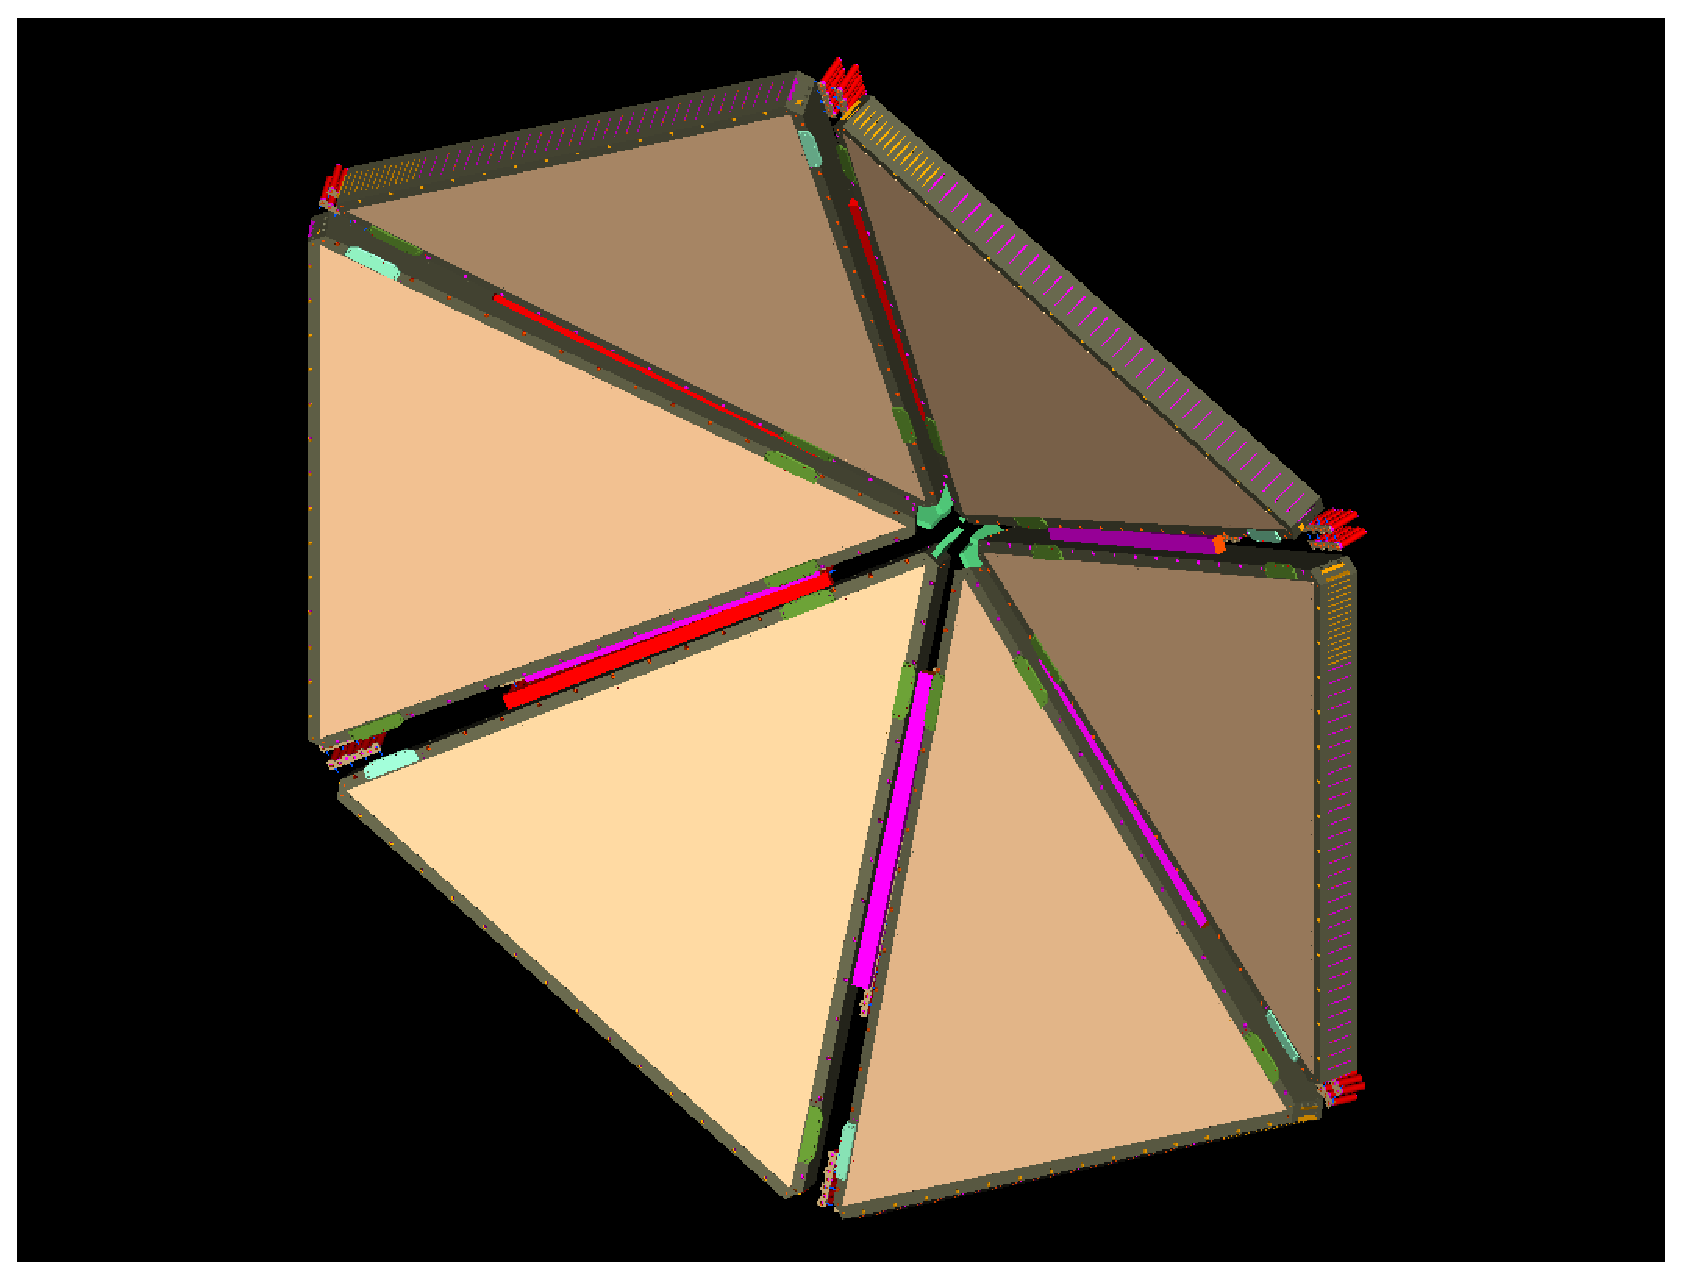
\epsfig{file=pcal_all_6.eps,width=14cm}
%%\end{center}
%%\end{figure}

\begin{center}
\Large Version 1.2
\end{center}


\pagestyle{empty}

\thispagestyle{empty}

\begin{center}
\title{DAQ and Trigger Systems for the CLAS12 detector}
\date{}


%\vskip 0.7cm
\maketitle


%%{\it{S.Boyarinov, C.Cuevas, E.Jastrzembski, S.Pozdnyakov \\}}
%%\smallskip
%%{\small{\jlab}}
%%\bigskip

%%{\it{C.Smith \\}}
%%\smallskip
%%{\small{\uvch}}
%%\bigskip

%%{\it K.Mikhailov, A.Vlassov\\}
%%\smallskip
%%{\small \itep}
%%\bigskip



\end{center}







\thispagestyle{empty}

\begin{abstract}

Document contains section `The CLAS12 detector Data Aquisition and
Trigger System' included into set of documents for July 2008 CD3 review.

\end{abstract}

\newpage
\tableofcontents

\newpage

\fancypagestyle{myheading}{%                % Redefining plain style
\fancyhf{} % clear all header and footer fields
\fancyhead[C]{\vspace{0.5cm}\line(1,0){500}\vspace{-0.5cm}}
\fancyhead[l]{\mbox{\bfseries CLAS12 Technical Design Report}}
\fancyhead[r]{\mbox{\bfseries Version 1.2 \date{\today}}}
\fancyfoot[C]{\mbox{\bfseries  \thepage }}
\fancyfoot[r]{\mbox{\bfseries DAQ and Trigger}}
\fancyfoot[l]{\vspace{-1cm}\line(1,0){500}}
}
\renewcommand{\headrulewidth}{0pt}
\renewcommand{\footrulewidth}{0pt}
\pagestyle{myheading}

%%

\section{Overview and Requirements}

\subsection{Requirements}

The following parameters are required for the {\tt CLAS12} Data 
Acquisition (DAQ) System: at least 10~kHz event rate, at least 100~MB/s 
data rate at the Event Recorder level, and not more than a 15\% dead 
time under the above listed conditions.

\subsection{Current DAQ System Analysis}

Currently the {\tt CLAS} DAQ system runs at an 8-10~kHz 
event rate and a 25-35~MB/s data rate at a dead time of not more than 
15\%.  Since it will be partially re-used in {\tt CLAS12}, we will 
discuss its main features and limitations, along with improvements 
necessary to achieve the {\tt CLAS12} requirements.

\subsubsection{Front-End Electronics: ADCs}

The currently used FASTBUS 1881M ADCs set a limit for the entire DAQ 
system: 12~$\mu$s conversion time projected into 12\% dead time at 10~kHz 
event rate.  It can be improved by switching to the low-resolution mode of
these units, which sets a 9~$\mu$s conversion time.  In this case the 
event rate limit can be pushed up to about 15~kHz.  This means that from 
a performance point of view, the 1881M ADCs can be re-used, however, the 
number of FASTBUS ADCs must be doubled to equip all new detectors, and 
delay cables and pretrigger discriminators must be purchased as well.

We have decided to replace all existing ADCs and equip all new detectors with
Flash ADC boards. That decision provides higher performance for the traditional
DAQ system and free-running DAQ compatibility for future upgrades.  Flash ADC
boards with on-board processing units will be used as the first stage of the
Level-1 trigger, so no pretrigger discriminators are required (as in the
current {\tt CLAS} DAQ system.  The delay cables will be eliminated as well.

It should be mentioned that removing the 1881Ms will increase the Level-1 
trigger decision time from hundreds of nanoseconds to at least 3~$\mu$s, 
making it more powerful.  In addition, Flash ADCs can deliver more 
detailed information to the trigger logic than the pretrigger discriminators.

\subsubsection{Front-End Electronics: TDCs and Discriminators}

All fast detectors in {\tt CLAS} are already equipped with new pipeline TDC
boards, both low (85~ps) and high (35~ps) resolution, and they will be
re-used in {\tt CLAS12}.  All new detectors will be equipped with the same
types of boards.  We are planning to purchase new VME-based JLAB-made
discriminators to equip all channels, eliminating the existing CAMAC-based 
LeCroy discriminators.

\subsubsection{Front-End Electronics: TDCs and ADBs in Drift Chambers}

The drift chamber readout is equipped with FASTBUS 1877 TDCs, and according 
to our plan, they will be re-used in {\tt CLAS12}.  All FASTBUS crates
needed to accommodate those TDCs were recently equipped with new remotely 
controllable power supplies and fan units, which will extend their lifetime. 
The LeCroy 1877 TDC board has the following basic parameters: 500~ns
resolution, 20~ns double-pulse resolution, up to 32~$\mu$s full scale, 
1 to 512~$\mu$s fast clear window with 250~ns fast clear settling time, 
conversion time 750~ns + 50~ns/hit (1.6~$\mu$s minimum). The conversion time
and readout speed of the 1877s will not limit the DAQ performance until about 
15~kHz, however, we may see aging effects and the necessity to increase the 
event rate beyond 15~kHz in the future.  In that case, all FASTBUS 1877
TDC boards can be replaced with pipeline TDCs. Replacement will not require 
any additional changes in other subsystems such as the trigger electronics.

The Amplifier-Discriminator board (ADB) electronics will be partially re-used,
but new ADB crate backplanes, multiplexer (MUX) boards, and trigger boards 
(segment finders) will be designed.  The number of ADB crates will be decreased 
from 30 to 18, leaving a significant number of spare power supplies and fan units.

\subsubsection{Trigger System}

The current {\tt CLAS} Level-1/Level-2 trigger system will be completely 
replaced with a new Level-1/Level-2 system capable of a few microseconds 
decision time.  The new trigger system will include segment and track 
finding capabilities in the drift chambers, cluster finding in the 
calorimeters, and matching capabilities between different detectors.  In
addition, a Level-3 trigger will be running between the Event Builder and 
the Event Recorder for additional event rate reduction and/or data
filtering.  Level-3 will perform full event reconstruction, including
hit-based tracking and time-based tracking, if required.  The trigger system, 
in general, will be flexible to accommodate different running conditions, 
with the main goal to search for events with electrons.

\subsubsection{Online Monitoring}

Four practically independent monitoring systems are currently used in 
{\tt CLAS}: Nagios-based computer and network monitoring, SmartSocket-based 
DAQ and Online monitoring, EPICS-based slow controls monitoring, and data 
monitoring.  In addition, a few smaller hardware-specific systems are used. 
The data monitoring system includes visualization only, with almost no alarm 
capabilities.

{\tt CLAS12} will have one integrated monitoring system, with a standard 
low-level interface compatible with the {\tt CLAS12} equipment.  It will 
also be compatible with the accelerator control and monitoring system on 
some level.  It will have not only monitoring, but also control capabilities. 
The implementation of such a system is under discussion and concept 
development will take at least one more year.  However, with our experience in 
developing and maintaining such systems, we are not expecting any problems in 
developing the new integrated system.

\subsubsection{Online Calibration}

The online calibration system must provide prompt information for the
trigger system and online monitoring, and will be used for preliminary
offline data processing.  Such a system does not exist in {\tt CLAS} and 
will be implemented in {\tt CLAS12}.

\subsection{`Free-Running' vs. Traditional DAQ Systems}

Since we will employ some old FASTBUS boards in the readout, the new
DAQ system cannot be run in `free-running' mode, however, all new components 
will be compatible with the `free-running' concept.  This means that the
{\tt CLAS12} DAQ system will become `free-running' after all FASTBUS boards 
are replaced in the future.

\subsection{SVT Readout}

The Silicon Vertex Tracker (SVT) is not a part of the {\tt CLAS12} trigger 
system.  The SVT readout is not included in the {\tt CLAS12} DAQ section, 
and is described in detail in the SVT section of this document (see
Section~\ref{svt:daq}.  However, it should be mentioned that the current SVT 
readout design sets a limit for the Level-1 trigger decision time at 3~$\mu$s, 
which may effect its ability to make the desired decisions.  Two solutions in 
the SVT readout are considered to avoid that problem: new readout chips and
a 16~$\mu$s Level-2 FIFO buffer.  More details can be found in the SVT section.










\section{Hardware Design}

\subsection{Overview}

The generic scheme for the {\tt CLAS12} DAQ system hardware is shown in 
Fig.~\ref{fig:HARDWARE1}.  This system will be described in detail in 
the following sections.

%%%%%%%%%%%%%%%%%%%%%%%%%%%%%%%%%%%%%%%%%%%%%%%%%%%%%%%%%%%%%%%%%%%%%%
\begin{figure}[ht]
\vspace{130mm}
\special{psfile=CLAS12_HARDWARE_1.eps hscale=60 vscale=60 hoffset=0 
voffset=0}
\caption{\small{Generic scheme for the {\tt CLAS12} DAQ system hardware.}}
\label{fig:HARDWARE1} 
\end{figure}
%%%%%%%%%%%%%%%%%%%%%%%%%%%%%%%%%%%%%%%%%%%%%%%%%%%%%%%%%%%%%%%%%%%%%%

\subsection{Front-End for Fast Detectors}

{\tt CLAS12} will have two calorimeters, two time-of-flight systems, and 
two {\v C}erenkov counters with more than 3700 total PMT channels. Every 
PMT will be connected to a Flash ADC and to a TDC through a discriminator 
(see Figs.~\ref{fig:TDC1} and \ref{fig:ADC1}).  Splitter panels will be used 
to deliver signals to both the ADC and TDC subsystems.  Four VME64X and 
nineteen VXS crates will be used to accommodate the 56 TDC and 244 ADC boards. 
Sixteen VME crates will contain the 262 discriminator boards.

The 16-channel JLab-made discriminators have a controllable threshold and 
output signal width.  They have built-in scalers, and every VME crate with
discriminators will have a readout controller (ROC), so those scalers can be 
read out.  The discriminators were successfully used in the {\tt CLAS} 
tagger system.  A new revision of the discriminators for {\tt CLAS12} will 
have a test input for calibration purposes and a channel mask.  This is
currently under development.

In {\tt CLAS12}, 128-channel 85~ps resolution and 32-channel 35~ps resolution 
pipeline TDCs will be used.  The first channel of every board will be 
connected to a reference signal through a discriminator to provide a timing 
reference.  The {\tt CLAS} system has been using these TDC boards for several 
years.  A recent firmware version for those TDCs has reached 160~MB/s
readout speed due to advanced 2eSST data transfer protocols.

%%%%%%%%%%%%%%%%%%%%%%%%%%%%%%%%%%%%%%%%%%%%%%%%%%%%%%%%%%%%%%%%%%%%%%
\begin{figure}[ht]
\vspace{130mm}
\special{psfile=CLAS12_TDC_1.eps hscale=62 vscale=62 hoffset=10 voffset=10}
\caption{\small{Planned scheme for the TDC readout in {\tt CLAS12}.}}
\label{fig:TDC1} 
\end{figure}
%%%%%%%%%%%%%%%%%%%%%%%%%%%%%%%%%%%%%%%%%%%%%%%%%%%%%%%%%%%%%%%%%%%%%%

The 16-channel JLab-made Flash ADCs are still under development and were 
not available for testing in {\tt CLAS} at the time of writing of this
document.  However, based on our tests with commercially available Flash 
ADC boards (Struck SIS3320, see Refs.~\cite{pozd,smith}), {\tt CLAS12} can 
be equipped with 12-bit 200~MHz boards. We are expecting that the JLab 
FADCs will satisfy those requirements.

The FADCs are a significant part of the trigger system and will send
prompt information to the Cluster Finder board installed in the same
crate. The cluster information will include energy for every channel above 
threshold.  A threshold will be applied to the energy sum of several 
consecutive hits.  Information will be sent to the Cluster Finder over the 
backplane serial bus every 16~ns.  The Cluster Finder board is described 
in Section~\ref{l1trig}, along with the energy summing algorithm.

%%%%%%%%%%%%%%%%%%%%%%%%%%%%%%%%%%%%%%%%%%%%%%%%%%%%%%%%%%%%%%%%%%%%%%
\begin{figure}[ht]
\vspace{130mm}
\special{psfile=CLAS12_ADC_1.eps hscale=60 vscale=60 hoffset=0 voffset=0}
\caption{\small{Planned scheme for the ADC readout in {\tt CLAS12}.}}
\label{fig:ADC1} 
\end{figure}
%%%%%%%%%%%%%%%%%%%%%%%%%%%%%%%%%%%%%%%%%%%%%%%%%%%%%%%%%%%%%%%%%%%%%%

\subsection{Front-End for the Drift Chambers}

The existing {\tt CLAS} preamplifier hybrid boards will be re-used for
sense wire signal amplification.  The existing MUX boards will be redesigned 
and the ADB crates will be equipped with new backplanes.  The ADB crates will 
be reused, probably with new power supplies installed.  Fig.~\ref{fig:ADB1} 
shows the new ADB electronics layout that is planned.  One ADB crate will have 
14 96-input preamplifier boards serving a complete drift chamber region, with 7 
boards per superlayer (112$\times$6 wires = 96$\times$7 channels).  The new MUX 
boards will send data to the new Segment Finder using a 96-wire bus and ECL
outputs to the TDCs after a 2-to-1 multiplexing.  The ADB crate backplane has 
two 96-line buses, one per superlayer, ending in the middle of crate, where the 
two-unit-wide Segment Finder is installed.  Communication between the various 
components is described in Section~\ref{l1trig}.

%%%%%%%%%%%%%%%%%%%%%%%%%%%%%%%%%%%%%%%%%%%%%%%%%%%%%%%%%%%%%%%%%%%%%%
\begin{figure}[ht]
\vspace{12.0cm}
\special{psfile=CLAS12_ADB_1.eps hscale=62 vscale=64 hoffset=15 voffset=0}
\caption{\small{Planned layout of an ADB crate for {\tt CLAS12}.}}
\label{fig:ADB1} 
\end{figure}
%%%%%%%%%%%%%%%%%%%%%%%%%%%%%%%%%%%%%%%%%%%%%%%%%%%%%%%%%%%%%%%%%%%%%%

18 ADB crates will be connected to 9 FASTBUS crates containing 14 LeCroy 
1877 TDC boards each.  The FASTBUS crates will be upgraded with new Wiener 
power supplies that include remote control.  In the future, the FASTBUS
electronics can be replaced by 6 VME64X crates containing 16 v1190
CAEN TDC boards each (see Fig.~\ref{fig:DC1}).

%%%%%%%%%%%%%%%%%%%%%%%%%%%%%%%%%%%%%%%%%%%%%%%%%%%%%%%%%%%%%%%%%%%%%%
\begin{figure}[ht]
\vspace{13.0cm}
\special{psfile=CLAS12_DC_1.eps hscale=64 vscale=64 hoffset=15 voffset=5}
\caption{\small{Schematic layout of the planned readout configuration
for the {\tt CLAS12} drift chambers.}}
\label{fig:DC1} 
\end{figure}
%%%%%%%%%%%%%%%%%%%%%%%%%%%%%%%%%%%%%%%%%%%%%%%%%%%%%%%%%%%%%%%%%%%%%%

In addition to aging problems, the FASTBUS TDCs may set another limitation 
for the {\tt CLAS12} DAQ system.  Currently they are programmed to accept 
up to 4 hits during a 2~$\mu$s interval, which corresponds to the maximum 
drift time in the Region~3 {\tt CLAS} drift chamber. The {\tt CLAS12} drift 
chambers will have similar drift times, so the TDC window will be set to similar 
values as with the current {\tt CLAS} configuration.  Unfortunately, with the 
FASTBUS 1877 TDCs, we can only program the window size against a common stop 
signal.  This signal is derived from the Level-1 trigger signal, and can be 
delayed a few microseconds to the TDC inputs.  In that situation, we have to open 
the TDC window by a few more microseconds, which may lead to more background 
hits.  In that case, we may need to allow 8 or 16 hits per channel to make 
sure that we are not losing useful hits.  That may increase the TDC conversion 
time (which is hit-dependent) and the data rate from the FASTBUS crates, which
would lead to a decrease in the overall DAQ performance.  Our backup VME-based 
solution will be activated if the FASTBUS electronics will not be usable for 
any reason.

\subsection{{\tt CLAS12} Trigger}

{\tt CLAS12} will have a three-level trigger system.  The Level-3 trigger 
is a software-based component and will be discussed in Section~\ref{sec:software}.  
The following sections contain a detailed description of the hardware-based 
Level-1 and Level-2 trigger components.

\subsubsection{Trigger Efficiency Study}

As a first step in the {\tt CLAS12} trigger system design, we studied the
efficiency of the current {\tt CLAS} trigger system.  In particular, we
studied its efficiency for electrons, which is important for most of the
physics program.  Detailed results can be found in Ref.~\cite{mikh}.
We found that by increasing the {\v C}erenkov counter pretrigger 
discriminator threshold up to 2 photoelectrons, we can make the electron 
trigger much more selective.  However, {\tt CLAS} has never run with that 
threshold because of the possibility of losing electrons with low energy 
deposition in the {\v C}erenkov counter.  {\tt CLAS12} will have two 
{\v C}erenkov counters, so even with a lower threshold, it is expected that
electron selection will be improved.  We also found that many non-electron 
events can be rejected by doing pattern recognition in the drift chambers 
and matching tracks with the fast detectors.  The new {\tt CLAS12} trigger 
system was designed to be flexible enough to exercise different approaches, 
depending on the particular run requirements.

\subsubsection{Trigger System Timing and Layout}

The maximum trigger decision time is currently set to 3~$\mu$s for Level-1
and 4~$\mu$s for Level-2.  The first number is defined by the SVT readout
chip, and the sum of both times must be less then 8~$\mu$s, which is defined 
by the FADC units.  Our preliminary FPGA algorithm development shows that 
3~$\mu$s for Level-1 may not be enough, for example, to complete the cluster 
finding in the calorimeters using energy corrections.  Those time constraints 
can be mitigated by using newer SVT readout chips and bigger FPGAs in the FADC
boards.

It is important to make sure that logically completed parts of the detector 
will not be wired to the several FPGAs inside the Cluster Finder boards, which 
will make cluster reconstruction much more difficult.  The current Cluster
Finder board design contains two FPGAs, which collect information from 8 FADC 
modules each.  That layout will satisfy all possible Level-1 algorithms.

\subsubsection{Level-1 Trigger}
\label{l1trig}

The Level-1 trigger system is based on fast detectors equipped with Flash
ADCs.  The first stage components of the trigger hardware are incorporated 
into the Data Acquisition elements (VXS crates), while the final decision is 
made in a specialized trigger crate containing Level-1 Subsystem
Processors. The same crate also contains Level-2 Road Finders and
Level-1/Level-2 matching logic incorporated into the Global Trigger
Processor, as well as Trigger Supervisor boards as 
shown in Fig.~\ref{fig:TRIGGER1}.  The system is driven by a 16~ns global
clock with an internal FPGA 4~ns clock.

%%%%%%%%%%%%%%%%%%%%%%%%%%%%%%%%%%%%%%%%%%%%%%%%%%%%%%%%%%%%%%%%%%%%%%
\begin{figure}[ht]
\vspace{145mm}
\special{psfile=CLAS12_TRIGGER.eps hscale=55 vscale=55 hoffset=0 voffset=0}
\caption{\small{Trigger system logic diagram for {\tt CLAS12}.}}
\label{fig:TRIGGER1} 
\end{figure}
%%%%%%%%%%%%%%%%%%%%%%%%%%%%%%%%%%%%%%%%%%%%%%%%%%%%%%%%%%%%%%%%%%%%%%

The VXS crates shown in Fig.~\ref{fig:ADC1} contain two trigger system
components: processing units on the FADC boards (Fig.~\ref{fig:TRIGGER_FADC})
and Cluster Finder (CF) boards that collect data from the Flash ADCs over fast 
serial lines.  The CF boards search for clusters in the electromagnetic 
calorimeters and other detectors, and send the results to the following 
stage of the trigger system (see Fig.~\ref{fig:TRIGGER_CF}).  A signal 
processing algorithm running in the FADC board processing unit is shown in 
Fig.~\ref{fig:TRIGGER_FADC_1}.

%%%%%%%%%%%%%%%%%%%%%%%%%%%%%%%%%%%%%%%%%%%%%%%%%%%%%%%%%%%%%%%%%%%%%%
\begin{figure}[ht]
\vspace{12.0cm}
\special{psfile=CLAS12_TRIGGER_FADC.eps hscale=62 vscale=64 hoffset=0 voffset=5}
\caption{\small{Processing unit on the FADC board.}}
\label{fig:TRIGGER_FADC} 
\end{figure}
%%%%%%%%%%%%%%%%%%%%%%%%%%%%%%%%%%%%%%%%%%%%%%%%%%%%%%%%%%%%%%%%%%%%%%

%%%%%%%%%%%%%%%%%%%%%%%%%%%%%%%%%%%%%%%%%%%%%%%%%%%%%%%%%%%%%%%%%%%%%%
\begin{figure}[ht]
\vspace{10.0cm}
\special{psfile=CLAS12_TRIGGER_CF1.eps hscale=20 vscale=25 hoffset=15 voffset=0}
\caption{\small{Cluster Finding diagram on the Cluster Finder board.}}
\label{fig:TRIGGER_CF} 
\end{figure}
%%%%%%%%%%%%%%%%%%%%%%%%%%%%%%%%%%%%%%%%%%%%%%%%%%%%%%%%%%%%%%%%%%%%%%

%%%%%%%%%%%%%%%%%%%%%%%%%%%%%%%%%%%%%%%%%%%%%%%%%%%%%%%%%%%%%%%%%%%%%%
\begin{figure}[ht]
\vspace{10.0cm}
\special{psfile=CLAS12_TRIGGER_FADC_1.eps hscale=60 vscale=60 hoffset=15 voffset=0}
\caption{\small{Signal processing algorithm on the FADC board.}}
\label{fig:TRIGGER_FADC_1} 
\end{figure}
%%%%%%%%%%%%%%%%%%%%%%%%%%%%%%%%%%%%%%%%%%%%%%%%%%%%%%%%%%%%%%%%%%%%%%

\subsubsection{Level-2 Trigger}

The ADB crates shown in Fig.~\ref{fig:ADB1} contain the Segment Finder 
(SF) boards that collect data from the set of drift chamber MUX boards
corresponding to an entire drift chamber region. The SF boards search for
track segments and send them onto the following stage.  The MUXs send data 
with a 15~ns strobe, so in a 105~ns interval, all data from both superlayers
is injected into a programmable delay (see Fig.~\ref{fig:TRIGGER2}).  The 
Level-1-driven switch and latch units accumulates the drift chamber hits 
during a 2~$\mu$s interval and passes the result to the Segment Finder board 
for processing.

The Segment Finder searches for segments in both superlayers simultaneously, 
then performs a region-based segment search, and finally builds a list of 
region-based segments.  The system works as a pipeline and sends sets of 
segments to the Level-2 Road Finders. Every segment occupies 24 bits: 7 bits for 
wire numbers in $U$ and 5 bits for the $U$-$V$ difference for the first and 
last wires in the region-based segment.

Six Level-2 Road Finder boards are installed in the trigger crate along with 
six Level-1 Subsystem Processor boards, a Global Trigger Processor (GTP) board, 
and a Trigger Supervisor (TS) board. The system collects all information from 
the fast detectors and drift chambers, along with the information from the 
central detectors.  It performs drift chamber-based track finding and matches 
the tracks with clusters from the fast detectors.  The Global Trigger Processor 
collects the data from the Level-1 Subsystem Processors and Level-2 Road Finders 
and produces the Level-2 trigger signals (see Fig.~\ref{fig:TRIGGER1}).

The Trigger Supervisor generates the Level-1/Level-2 pass/fail and other 
signals, and controls the entire DAQ system readout through the Trigger 
Interface units.  The Trigger Interface (TI) units installed in every 
crate participate in the readout process.

\subsubsection{Level-1/Level-2 Timing Diagram}

The generic scheme for the Level-1/Level-2 trigger timing is shown in 
Fig.~\ref{fig:TRIGGER2}.  The entire trigger system can be considered as a
three-stage process.

The first stage is the Level-1 sector-based trigger, which includes the FADC 
on-board processing (T1), data transfer over the VXS backplane serial bus (T2), 
cluster finding (T3), data transfer to the trigger crate (T4), sector-based 
Level-1 decision (T5), and data transfer to the following trigger stages.  
During that period of time (T1+T2+T3+T4+T5+T6+T7), the drift chamber signals are 
delayed by a programmable delay on the MUX boards in the ADB crates.  The T3 and 
T5 time intervals can be different for different run periods, so the programmable 
delay must be reprogrammed accordingly.

The second stage starts when the Level-1 signal arrives at the ADB crate, 
initiating the drift chamber hit-latching process (T8).  The typical T8 
timing is about 2~$\mu$s and is defined by the maximum drift time.  Three 
latch units will be used for every channel, so up to three Level-1 triggers 
can be processed in parallel.  If a fourth Level-1 signal arrives while 
the first one is still latching, the whole trigger system will be stopped, 
however, such events will be extremely rare based on the expected trigger
rate.  After the latching process is finished, the latched hits will be 
transferred to the Segment Finder (T9), processed there (T10), and the list
of segments will be transferred to the Level-2 Road Finders (T11) installed in 
the trigger crate, and processed there (T12).  During that period of
time (T8+T9+T10+T11+T12), the Level-1 information (clusters from the
Level-1 Subsystem Processors) will be delayed by another programmable delay.

Stage three is the final Level1/Level2 trigger processing stage in the
Global Trigger Processor (T13+T14) and Trigger Supervisor (T15). The
total trigger decision time must be less than 7~$\mu$s to satisfy
the Flash ADC range.

%%%%%%%%%%%%%%%%%%%%%%%%%%%%%%%%%%%%%%%%%%%%%%%%%%%%%%%%%%%%%%%%%%%%%%
\begin{figure}[ht]
\vspace{12.0cm}
\special{psfile=CLAS12_TRIGGER_2.eps hscale=58 vscale=58 hoffset=10 voffset=0}
\caption{\small{Level-1 and Level-2 trigger timing diagram.}}
\label{fig:TRIGGER2} 
\end{figure}
%%%%%%%%%%%%%%%%%%%%%%%%%%%%%%%%%%%%%%%%%%%%%%%%%%%%%%%%%%%%%%%%%%%%%%

\subsection{Readout Controllers}

Readout Controllers (ROCs) are installed in every FASTBUS, VME, VME64X, 
and VXS crate.  The ROCs collect data from the front-end boards, process it, 
and send it to the Event Builder over the network.  Currently we employ 
mvme6100 controllers with a prpmc880 or pmc280 co-processor module.  That 
configuration is fast enough to meet the {\tt CLAS12} requirements and more 
co-processor modules can be installed if necessary.  By the time of 
{\tt CLAS12} startup, a new generation of ROCs (including multi-processor and 
multi-core units) will be available.

\subsection{Computing and Network}

A Foundry 1500 switch is currently used as the backbone of the DAQ system, 
and a similar switch will be used for {\tt CLAS12}.  The Event Builder, 
Event Recorder, and other critical DAQ components for {\tt CLAS} are 
running on 4-CPU Opteron-based servers, and that configuration is sufficient 
for {\tt CLAS12} as well.  ROCs are linked to the 1500 Foundry switch
through smaller switches with up to four GBit uplinks (see Fig.~\ref{fig:NET1}).  
The {\tt CLAS} data storage system (RAID5) is sufficient for up to a 150~MB/sec 
data rate.

All available equipment is good enough to satisfy the {\tt CLAS12} 
requirements, but most likely we will upgrade most of the components 
because of aging and maintenance considerations.  The performance of the 
link to the JLab Computer Center tape storage must be increased
up to at least 200~MB/s.

%%%%%%%%%%%%%%%%%%%%%%%%%%%%%%%%%%%%%%%%%%%%%%%%%%%%%%%%%%%%%%%%%%%%%%
\begin{figure}[ht]
\vspace{12.0cm}
\special{psfile=CLAS12_NET_1.eps hscale=64 vscale=64 hoffset=10 voffset=5}
\caption{\small{Planned scheme for {\tt CLAS12} networking.}}
\label{fig:NET1} 
\end{figure}
%%%%%%%%%%%%%%%%%%%%%%%%%%%%%%%%%%%%%%%%%%%%%%%%%%%%%%%%%%%%%%%%%%%%%%

\section{Software}
\label{sec:software}

\subsection{CODA Data Acquisition System}

{\tt CLAS12} will use the CODA data acquisition software~\cite{coda}, similar 
to what we are using in {\tt CLAS}.  The {\tt CLAS} version of CODA was 
modified in recent years to improve performance and reliability, and those 
changes will be incorporated into the future version of CODA, along with 
appropriate redesign and cleanup.  The most important changes were `parallel' 
front-end readout, multi-processor ROC support, and a multi-threaded Event 
Builder.  As a result, {\tt CLAS} is running at an 8-10~kHz event rate, 
which is close to the {\tt CLAS12} requirements.  We are expecting to get 
new software from the CODA group by the time of {\tt CLAS12} startup.  Until
then, we will use the current {\tt CLAS} version of CODA for detector 
commissioning and test runs.

Recent upgrades have eliminated most of bottlenecks from the DAQ software, but 
there are still places where improvements can be made.  One of them is 
multi-event readout and corresponding data coping inside the ROC memory. 
That modification will improve DAQ performance significantly for the 
free-running DAQ mode, but it will not have a big impact while {\tt CLAS12}
is using FASTBUS 1877 TDCs. Those TDCs have 6 event buffers and need to be
readout on an event-by-event basis to avoid back-logs.  When the FASTBUS 
electronics are replaced, we plan on utilizing multi-event readout.

\subsection{{\tt CLAS12}-Specific Components Running as CODA Extensions}

Several CODA extensions were developed for the {\tt CLAS} detector, and some 
of them will be re-used in {\tt CLAS12}.  The CODA fragment format was 
expanded by adding an additional data bank header; this way several data 
banks with different formats could be created and processed by the same ROC. 
This feature may be implemented into the new CODA version, or we can continue
to use it as it is implemented now.

The currently used BOS data format will be obsolete, and the CODA data format 
will be used instead for all output data files, but data will be organized 
based on the detectors, not on the readout hardware layout.  Again, it can 
be done by expanding the CODA format or by {\tt CLAS12}-specific extensions.

The data translation procedure running in the ROCs will be re-used, with 
possible data format modifications.  Two advantages of this method should 
be mentioned: the data volume reduction (especially in the drift chambers) 
and the ability to access data using the `offline' format on the very first 
stage of the data acquisition process.  Also the ROC-level histogram package 
played a critical role in the DAQ performance analysis, and it will be reused 
after adjustment to the new data format.  The DAQ performance profiler will 
be reused, although it may be part of the new CODA version as well.

The Event Transfer (ET) system in {\tt CLAS} was extended by adding a new 
package to handle multi-threaded attachments to a single ET station, with 
special care taken for preserving the event order.  This method was 
successfully used by the Event Builder, Level-3, and the fast online 
reconstruction software running on an 8-CPU Sparc Server, and will be 
reused in some form in {\tt CLAS12}.

\subsection{Level-3 Trigger}
\label{daq_l3t}

A multi-threaded Level-3 (software) trigger was implemented in {\tt CLAS}, 
but was used in tagging-mode only. We will redesign that component for 
{\tt CLAS12}, implementing full reconstruction up to at least the hit-based 
tracking level.  A single multi-core machine is used right now to run the
Level-3 trigger, and a computer farm solution can be used for {\tt CLAS12} 
if needed.

\subsection{Online Monitoring}

Online Monitoring will be addressed in {\tt CLAS12} as a part of the
Experiment Control System (ECS) concept.  This approach was used in 
previous years by other collaborations.  We will use their experience to 
design the {\tt CLAS12} ECS.

ECS will collect all information coming from various {\tt CLAS12} components
into one processing center, which will perform analysis and report problems 
with maximum possible precision.  To make the whole system work successfully,
all information from the low-level components will be reported in standard 
form, EPICS-channel access format is currently being considered.  Special 
care will be taken to avoid false alarms.

The generic scheme for the {\tt CLAS12} Experiment Control System is shown 
in Fig.~\ref{fig:MON1}.  Low-level hardware and data quality control 
components will communicate with top-level state machines using EPICS channel 
access and/or similar protocol.  The data acquisition components will have 
a DAQ-specific communication system.  Most state machines will be 
detector-specific, with one central component supervising the entire 
{\tt CLAS12} setup. A set of logic diagrams will be developed to handle 
different situations during {\tt CLAS12} experiments, such as production 
data taking, calibration runs, test runs, troubleshooting, recovery, etc. 
These diagrams will be processed by the state machines.

%%%%%%%%%%%%%%%%%%%%%%%%%%%%%%%%%%%%%%%%%%%%%%%%%%%%%%%%%%%%%%%%%%%%%%
\begin{figure}[ht]
\vspace{100mm}
\special{psfile=CLAS12_MON_1.eps hscale=64 vscale=64 hoffset=0 voffset=0}
%%\mbox{
%%\begin{picture}(-10,-10)(350,0)
%%\end{picture}}
\caption{\small{Generic scheme of the {\tt CLAS12} Experiment Control System.}}
\label{fig:MON1} 
\end{figure}
%%%%%%%%%%%%%%%%%%%%%%%%%%%%%%%%%%%%%%%%%%%%%%%%%%%%%%%%%%%%%%%%%%%%%%

The Experiment Control System for {\tt CLAS12} is currently under development.
We are looking into several frameworks that can be used to build the
{\tt CLAS12} ECS, such as CERN PVSS (used by all major CERN experiments), 
AFECS (under development at JLab), and others.

It may take a while to complete the design because of the dependency on 
the accelerator's control system, which we have to be compatible with on 
some level.  Several approaches are being considering by other JLab groups, 
and we are planning to participate in joint efforts to obtain the system
most suitable for {\tt CLAS12}. 

\subsection{Online Calibration}

The main goal of the online calibration system is to deliver the calibration 
parameters for the trigger components.  Normally, special runs will be taken 
and analyzed online before production data taking starts.  Those runs will be 
processed and analyzed by software included into the Level-3 trigger 
component running in tagging mode.

\section{Conclusion}

Since the current {\tt CLAS} DAQ system already has a performance close 
to that needed for {\tt CLAS12}, we are confident that the {\tt CLAS12} 
goals will be achieved with available solutions.  All new components
designed by the JLab CODA group and the JLab Fast Electronics Group for Hall~D
will be utilized in {\tt CLAS12}, since the {\tt CLAS12} requirements have
already been taken into account.







%%
\begin{thebibliography}{99}


\bibitem{coda} CODA DAQ System. 

\bibitem{clas} CLAS DAQ System. 

\bibitem{pozd} S.Pozdnyakov, CLAS-Note 2006-023. 

\bibitem{smith} C.Smith, CLAS12-Note 2007-xxx. 

\bibitem{mikh} K.Mikhailov, CLAS-Note 2007-009. 


\end{thebibliography}



\end{document}
























